In this section, 4 categories of attributes are defined using two concepts from fuzzy logic. Our approach will be to define these properties for each intervention.

First we define a fuzzy linguistic variable for each attribute. In the case of distances (between interventions and between parks and interventions), we will assign its values using fuzzy numbers, in specific trapezoidal and triangular fuzzy numbers (see figure \ref{fig:fuzzy_distance}). On the other hand, memberships to degrees of size and degrees of risk will be assigned via fuzzy cmeans, where each intervention may have multiple non-zero membership degrees to different clusters, their centroids can be seen in table \ref{tab:fuzzy_centroids}.

\begin{table}[!ht]
    \centering
    \begin{tabular}{lcc}
    \hline
    \textbf{Cluster Type} & \textbf{Size Centroids} & \textbf{Risk Centroids} \\
    \hline
    Small/Low & 389.36 & 972.16 \\
    Mid-small/Mid-low & 4,616.21 & 987.10 \\
    Medium/Mid & 8,304.83 & 997.60 \\
    Mid-large/Mid-high & 12,653.61 & 1,009.31 \\
    Large/High & 23,279.25 & 1,024.11 \\
    \hline
    \end{tabular}
    \caption{Fuzzy cluster centroids for intervention size and risk levels.}
    \label{tab:fuzzy_centroids}
    \end{table}
    
    
    \begin{figure}[!ht]
    \centering
    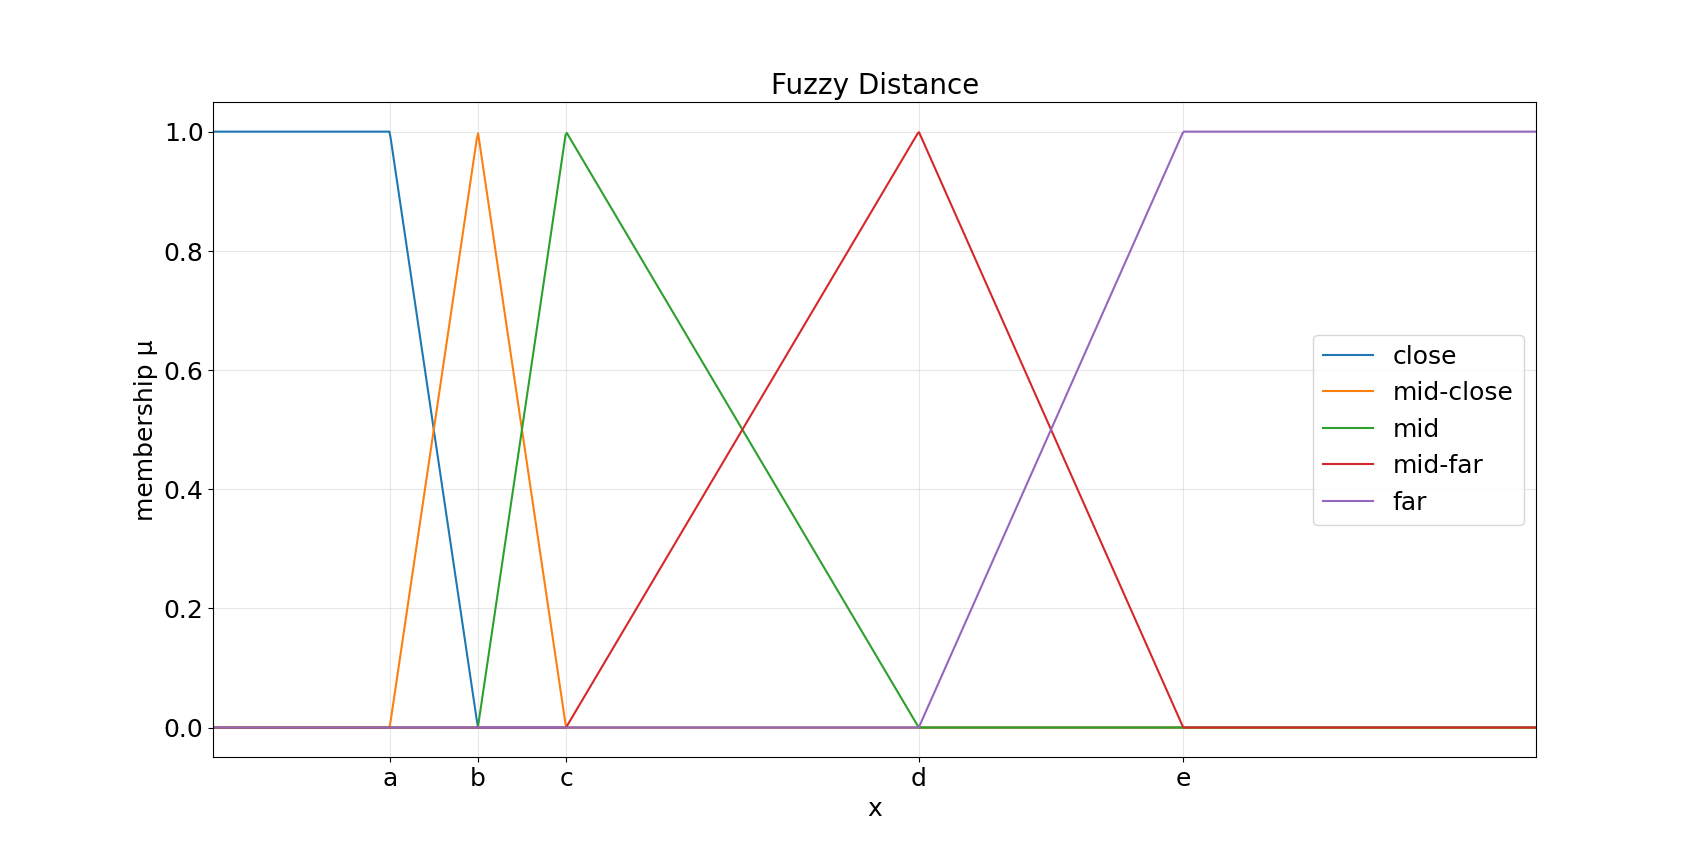
\includegraphics[width=\linewidth]{ch3/figures/Fuzzy distance.png}
    \caption{Fuzzy distance linguistic variable with close, mid-close, mid, mid-far and far membership functions.}
    \label{fig:fuzzy_distance}
    \end{figure}

In order to go from the membership values of interventions to membership values of a particular solution, we will leverage the distribution of daily masses of memberships over the planning horizon.

The idea is the following:

In the case of the distance matrix of distances intervention to intervention. We start by applying the fuzzy variable to the crisp distance matrix. This is a mapping from a real valued distance to 5 membership values, which can be represented with 5 matrices, one for each fuzzy distance (intervention to intervention) set. This are 5 fuzzy sets over the pairs of interventions. Afterwards, to compute the daily mass of each of those 5 fuzzy sets, we are going to take the cardinality of the each of those 5 fuzzy sets restricted to the unique pairs of active interventions in a day. Do this for each day in the time horizon. After that, we have a unique mass value for each day (see figure \ref{fig:fuzzy_att_concurrency}). 

In the case of the distance matrix from interventions (rows) to parks (colums). The approach is similar, we apply a different fuzzy distance variable and get 5 matrices. But in this case, since columns represent parks instead of interventions, we aggregate row wise each matrix using a t-conorm which converts each of the five matrices into a vector which corresponds to a five closeness to park value per intervention. Which are 5 closeness to park membership vectors (a fuzzy set over the set of interventions). Then the approach to generate the daily masses is analogous to the previous case. We take the fuzzy subset corresponding to the active interventions in any given day and add their memberships (cardinal of that fuzzy subset).

Regarding the risk and size, we have a mean size and a mean risk for each intervention (a vector). This is then fuzzy clustered into 5 clusters, therefore converting each vector of mean values into 5 vectors of memberships. Then the daily masses are computed analogously to the vectors from the distances to parks.

 

\begin{figure}[!ht]
    \begin{adjustwidth}{-1.6cm}{-1.6cm}
    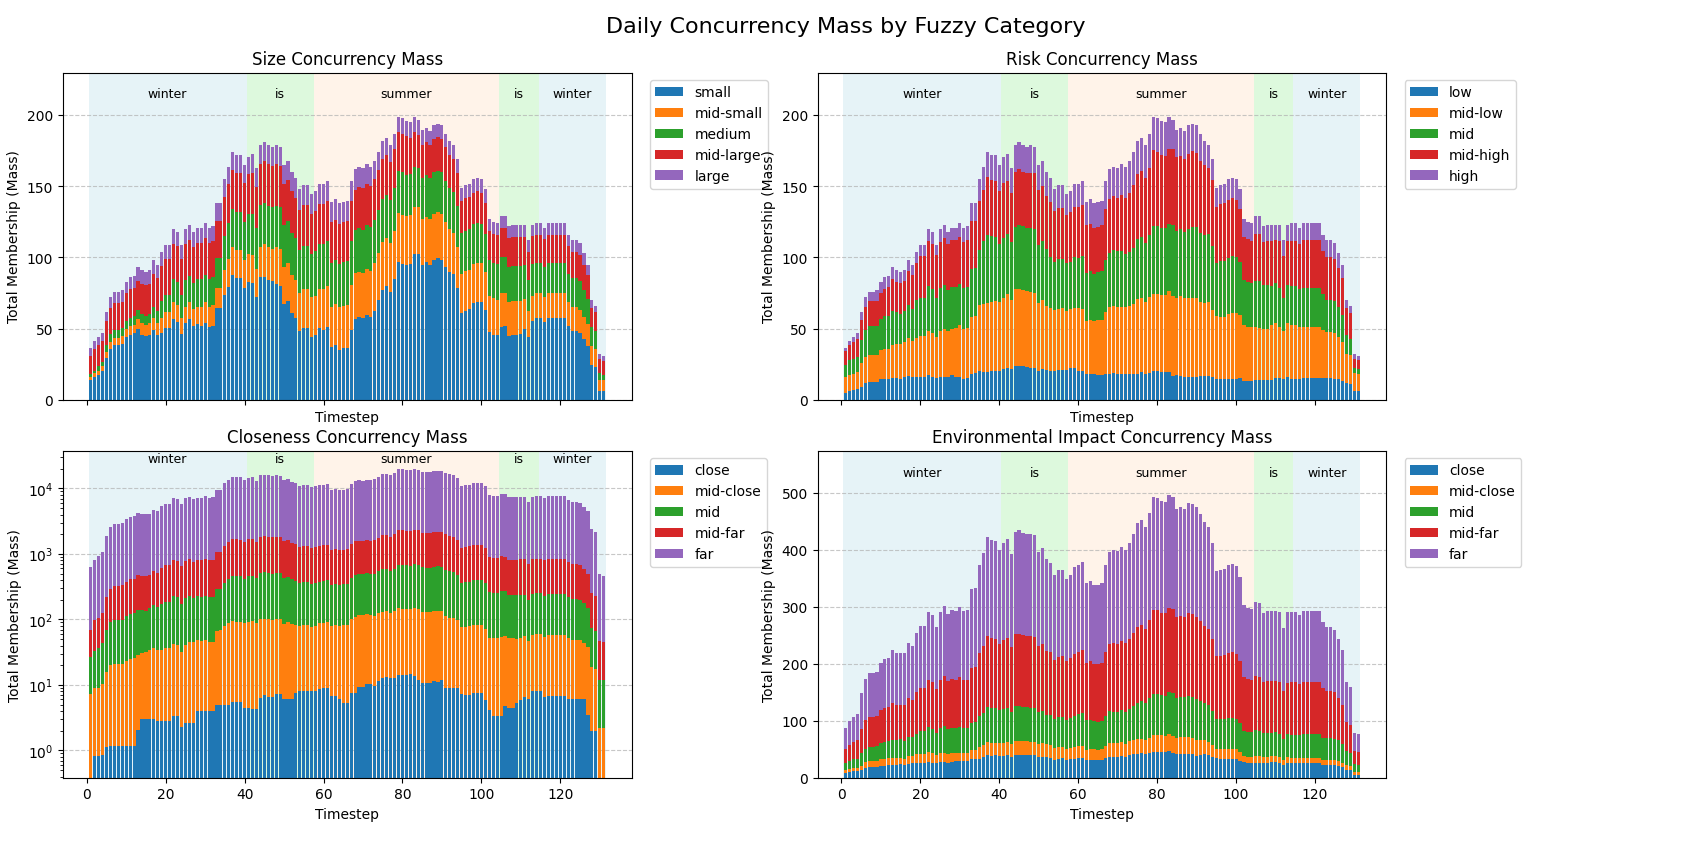
\includegraphics[width=1.07\linewidth]{ch3/figures/Fuzzy_att_concurrency.png}
    \end{adjustwidth}
    \caption{Distribution of daily masses of membership for an example solution throughout the planning horizon.}
    \label{fig:fuzzy_att_concurrency}
\end{figure}



\paragraph{Closeness Concurrency:} This attribute quantifies the degree to which interventions that are spatially "close" occur simultaneously. At each timestep \(t\), let \(\mathcal{I}(t)\) be the set of interventions active. For every unique pair \(\{i,j\}\) in \(\mathcal{I}(t)\), we...


\paragraph{Environmental Impact Concurrency:} This score quantifies the level of simultaneous interventions with different degrees of environmental impact over the planning horizon. At each timestep \(t\), let \(\mathcal{I}(t)\) denote the set of active interventions. 

\paragraph{Size Concurrency:} This attribute quantifies the degree of overlap among interventions with significant workload sizes. 

First, we compute the \textbf{mean intervention size}: For each intervention \(i\), we consider all possible start times \(\tau\). For each start time \(\tau\), the total workload is used to compute the mean intervention size for intervention \(i\):

\[
    \text{mean\_size}_i \coleq \frac{1}{|\mathcal{T}_i|} \sum_{\tau\in \mathcal{T}_i} \text{size}_{i,\tau},
    \qquad \text{with }\,
    \text{size}_{i,\tau} \coleq \left(\sum_{c \in C} \sum_{t=1}^{T} r_{c,t}(i,\tau)\right) \times d_{i,\tau}, \,\, \mathcal{T}_i = \{ \tau \mid \text{size}_{i,\tau} > 0 \}
\]

where \(C\) is the set of resources, \(r_{c,t}(i,\tau)\) is the consumption of resource \(c\) at time \(t\) when intervention \(i\) starts at \(\tau\), and \(d_{i,\tau}\) is the duration. Only start times with non-zero \(\text{size}_{i,\tau}\) are considered. 


Then, interventions are clustered into \texttt{small}, \texttt{mid-small},\texttt{mid}, \texttt{mid-large} and \texttt{large} groups using fuzzy cmeans on their mean intervention sizes. At each timestep \(t\), let \(\mathcal{I}(t)\) denote the set of active interventions. 

\paragraph{Risk Concurrency:} Analogous to size concurrency, risk concurrency quantifies the degree of overlap among interventions with elevated risk levels. In this case, each intervention \(i\in I\) has a risk value which is the average of its nonzero risk values $r_t^{(i)}$ (see Assumption 1) across all start times. Then, interventions are clustered via fuzzy cmeans into... The score is completely identical to the one from size concurrency.




Finally, each daily mass distribution (we have 5 linguistic values $\times$ 4 linguistic variables = 20 mass distributions). 

Since the total mass is the same for all the solutions (they all have to schedule the exact same interventions) and what varies is how that mass is distributed across the time horizon. We are going to consider that what would be best is to have those masses uniformly distributed and what would be worse is to have a peak day where all the dangerous, risky, huge and concentered in one place interventions, take place. With this intention we are going to normalize each distribution by their total mass (the shape of the distribution remains the same) and then take the minus entropy of that distribution.

Notice that here, we do not have any probabilities and entropy only serves as a measure of how uniformity. No information or probabilistic interpretation would make sense in this case.

In their foundational work, Cover and Thomas define the entropy $H(X)$ of a discrete random variable $X$ as a measure of uncertainty or randomness associated with the possible outcomes \cite[Section 2.1]{Entropy}. The entropy is calculated by the following formula:
\[
H(X) = - \sum_x p(x)\, \log p(x)
\]
where $p(x)$ denotes the probability of outcome $x$.

According to Cover and Thomas \cite[p.~14]{Entropy}, entropy is minimized when the distribution is deterministic, meaning that a single outcome has probability one and all others have probability zero. In this case, $H(X)=0$, reflecting the absence of uncertainty. Conversely, entropy is maximized by the uniform distribution. Specifically, for a variable $X$ with $|X|$ possible outcomes, the entropy satisfies the inequality
\[
H(X) \leq \log |X| 
\]
with equality if and only if $X$ is uniformly distributed \cite[Theorem 2.6.4, p.~27]{Entropy}. Therefore, a uniform distribution corresponds to maximum entropy, while a deterministic distribution yields the minimum possible entropy.

